%%%%%%%%%%%%%%%%%%%%%%%%%%%%%%%%%%%%%%%%%%%%%%%%%%%%%%%
%                   File: OSAmeetings.tex             %
%                  Date: 20 September 2021            %
%                                                     %
%     For preparing LaTeX manuscripts for submission  %
%       submission to Optica meetings and conferences %
%                                                     %
%       (c) 2021 Optica                               %
%%%%%%%%%%%%%%%%%%%%%%%%%%%%%%%%%%%%%%%%%%%%%%%%%%%%%%%

\documentclass[letterpaper,10pt]{article} 
%% if A4 paper needed, change letterpaper to A4

\usepackage{osameet3} %% use version 3 for proper copyright statement

%% standard packages and arguments should be modified as needed
\usepackage{amsmath,amssymb}
\usepackage{amsthm}
\usepackage[colorlinks=true,bookmarks=false,citecolor=blue,urlcolor=blue]{hyperref} %pdflatex
%\usepackage[breaklinks,colorlinks=true,bookmarks=false,citecolor=blue,urlcolor=blue]{hyperref} %latex w/dvipdf

\DeclareMathOperator*{\argmax}{arg\,max}
\DeclareMathOperator*{\argmin}{arg\,min}

\usepackage[english]{babel}
\newtheorem{theorem}{Theorem}
\newtheorem{corollary}{Corollary}
\newtheorem{lemma}[theorem]{Lemma}
\newtheorem{conjecture}{Conjecture}
\newtheorem{definition}{Definition}
\newtheorem{workdefinition}{Working Definition}
\newtheorem{problem}{Problem}
\newtheorem{example}{Example}
\newtheorem{remark}{Remark}

% \usepackage{color}
\usepackage[dvipsnames]{xcolor}
\newcommand\dashto{\mathrel{
  -\mkern-6mu{\to}\mkern-20mu{\color{white}\bullet}\mkern12mu
}}

\newcommand\indep{\perp \!\!\! \perp}

\usepackage{graphicx,centernot}
\newcommand{\CI}{\mathrel{\perp\mspace{-10mu}\perp}}
\newcommand{\nCI}{\centernot{\CI}}

% Usage
% $a \CI c \mid b$ and $a \nCI c \mid b$

\newcommand\R{\mathbb{R}}

\usepackage{caption}
\usepackage{subcaption}

\usepackage{dot2texi}

\usepackage{tikz}
% \usetikzlibrary{shapes,arrows}
\usetikzlibrary {graphs}

\newcommand\E{\mathbb{E}}




\begin{document}

\title{Inner Alignment through the lens of Causality: Initial Takeaways}

\author{David Reber}
\address{Columbia University}
\email{david.reber@columbia.edu}
%%Uncomment the following line to override copyright year from the default current year.
\copyrightyear{2022}


\begin{abstract}
abstract
\end{abstract}

%%%%%%%%%%%%%%%%%%%%%%%%%%%%%%%%%%%%%%%%%%%%%%%%%%%%%%%%%%%%%%%%%%%%%%%%%%%%%%%%%%%%%%%

\subsection{Intended Audience}
This post assumes prior familiarity with inner alignment; in particular, you've read at least two of \textcolor{red}{post A, post B, or post C}. Furthermore, basic familiarity with causal graphs; you've read The Book of Why, \textcolor{red}{these posts}, or better yet, \cite{pearl_2009}.

\section{Introduction}
Every researcher knows that the language you use is itself a modeling choice.
To paraphrase the oft-cited quote: `Every language has blindspots, but some are useful.'
Here, I present one possible mathematical formalism of inner alignment, some important implications and open questions that immediately follow, while tallying up the total cost of assumptions (blindspots) that are incurred along the way.

\section{What is inner alignment?}
Thus far, the extent to which inner alignment has been mathematicized appears to be in the following two lines:
\begin{align}
\theta^* &= \argmax_\theta \E(O_b(\pi_\theta)) \\
\pi_\theta &= \argmax_\pi \E(O_m(\pi|\theta))
\end{align}
where $O_b$ and $O_m$ are the base- and mesa-objective functions, inputting a policy $\pi_\theta$ and $\pi$ (after $\theta$ has been fixed), respectively \textcolor{red}{(cite)}.
This represents the dual optimization process of the base optimizer trying to find the best parameters for a mesa optimizer, to maximize the base objective (while the mesa optimizer is itself optimizing the mesa objective).
Alternatively, you can think of expressing these as a system of equations expressing that mesa-optimization has arisen, analogous to calculus' necessary first-order conditions satisfied at every critial point. \textcolor{green}{(extra:A)}.

\section{Current language of choice: Causality}

What are the causal concepts we'll use to express (and then expore) inner alignment?

\begin{itemize}
  \item causal graph
  \begin{itemize}
    \item exogeneity
    \item causal dependence
  \end{itemize}
  \item soft interventions
  \begin{itemize}
    \item $\sigma$-calculus
  \end{itemize}
  \item transportability
  \begin{itemize}
    \item selection diagram
  \end{itemize}
  \item (structural learning)
  \begin{itemize}
    \item equivalence classes of causal diagrams
  \end{itemize}
  \item (sensitivity analysis)
\end{itemize}

\textbf{Assumption:} We're going to assume acyclicity for now. (I have inside-view reasons to believe the analysis will extend naturally to cyclic systems as well).

\subsection{Mesa Optimization: Soft Interventions}

\begin{figure}
\centering
\begin{subfigure}{.5\textwidth}
  \centering
    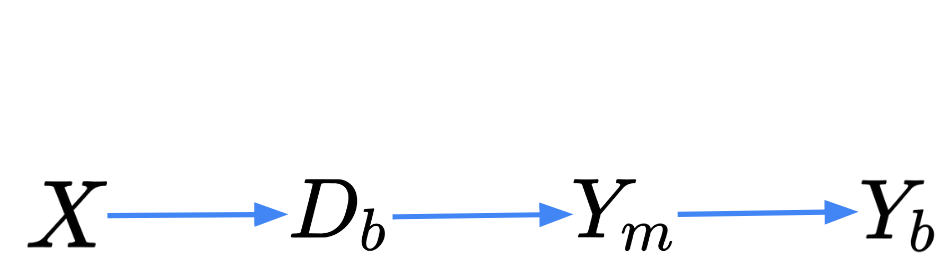
\includegraphics[width=.6\linewidth]{pics/my_own/minimal_aligned.png}
    \caption{minimal aligned}
    \label{fig:minimal-aligned}
\end{subfigure}%
\begin{subfigure}{.5\textwidth}
  \centering
    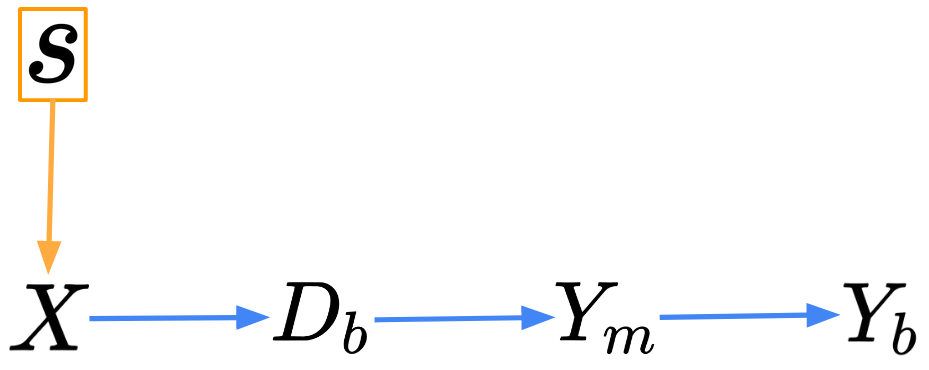
\includegraphics[width=.6\linewidth]{pics/my_own/minimal_selection.png}
    \caption{selection}
    \label{fig:minimal-selection}
\end{subfigure}
\caption{caption}
\label{fig:selection}
\end{figure}

\subsection{Inner alignment as a question of transportability}

A simple regime indicator $s$ is simply: "Are we in training right now?".

\textcolor{green}{(Extra:B, Extra:C, Main:1, Main:2, Main:3, Main:4)}

We say that the mesa-optimizer $D_m$ is \emph{inner aligned} if 
\[
\E(Y_b|Y_m,s,\sigma_{D_m}) = \E(Y_b|Y_m,\sigma_{D_m})
\]
This seems like the right definition because 
\begin{enumerate}
  \item Even though we can't measure $Y_m$ directly, we know it will always be maximally high
  \item The right-hand side is precisely the optimal expectation achieved during training
\end{enumerate}

A sufficient \textcolor{red}{(and necessary?)} condition for this to hold is if Rule 1 of the $\sigma$-calculus holds:
\[
(Y_b\indep s|Y_m)_{G_{\sigma_{D_m}}}
\]
That is, if $Y_m$ d-separates $Y_b$ from the regime change, we get robustness; we can reliably trust the mesa optimizer to help us achieve high $Y_b$ (at least, as well as it's capabilities allow...aka. intent alignment?).
\textcolor{green}{Extra:D}

I believe a necessary-and-sufficient condition for $(Y_b\indep s|Y_m)_{G_{\sigma_{D_m}}}$ is (excluding trivial cases like no causal connection whatsoever):
\begin{enumerate}
  \item $Y_b$ must be causally dependent on $Y_m$
  \item All causal paths from $s$ to $Y_b$ must pas through $Y_m$
\end{enumerate}
\textcolor{green}{Extra:E, Extra:F}.

Which situations pass this criteria, which don't? \textcolor{green}{(Extras: H - L)}

\subsection{What does $(Y_b\indep s|Y_m)_{G_{\sigma_{D_m}}}$ mean practically?}
As in, how could we empirically test it?

\begin{itemize}
  \item if we know $Y_m$, then knowing $s$ doesn't give us any more info about $Y_b$.
  \item if we know $Y_m$ is maximized then $Y_b$ is also maximized (thanks to the mesa-equations). \textcolor{red}{or is it just that the performance won't be worse than in training? Not necessarily better?}
\end{itemize}

\subsection{Speculation towards a plausible experiment}
If
\begin{enumerate}
  \item only the data is subject to regime shift,
  \item \textcolor{red}{....}
\end{enumerate}
Then $(Y_b\indep s|Y_m)_{G_{\sigma_{D_m}}} \iff (Y_b\indep data|D_b)_{P(V)}$?
(if so, then perhaps we can evaulate this during/after training?).

Furthermore, if some subset of the data satisfies the required independence relation, then we are robust w.r.t distributional shift in those dimensions.

\textcolor{red}{Finite data considerations? how to practically test the independence?}

\section{Sensitivity analysis}
So far, this has all been about enforcing a very strict equality. 
If however, we allow a mere bound (dependent on $Y_m$) like $Y_b$ is always 90 percent of optimal" then we might be able to do partial-identifiability; be able to run simulations just using the data/reward correlations (without needing the optimal policy), etc.

If we're willing to provide a parametrization of the world, then we can do sensitivity analysis! (Possible parametrizations: linear regression. Graph-constrained NN).

This would look like "Assuming this is the mesa objective function, how sensitive is $Y_b$ to a small regime change in the data?"
(And then perhaps we can try to encourage `nicer' mesa-objectives? soft inner alignment)

\section{musings}
I wonder if it's possible to numerically simulate the (likelihood? feasibility? magnitude?) of inner alignment as follows:
(data $\rightarrow D$, D is parent of both $Y_b$ and $Y_m$)
For a given mesa objective, does the correlation (data,high-$Y_m$, high-$Y_b$) exist? Is it a common occurance?
If so, how does the feasibility/frequency change as we gradually introduce a regime change to the data?


\section{Would you rather? The Wireheading / Inner Misalignment tradeoff}
We could perhaps force $D\rightarrow Y_m\rightarrow Y_b$by explicitly making reward depend on neuron values, etc. But won't this introduce a control incentive??

More generally, I wonder if $(Y_b\indep s|Y_m)_{G_{\sigma_{D_m}}}$ is really getting at \textbf{a fundamental tradeoff between wireheading and inner misalignment}, if both boil down to whether or not a path exists? (hopefully there's some cases missing - this is just intution speaking, haven't actually written it all out yet).

Even if this is the case, perhaps the effect of each could be attuned, so that we find a sweet-spot in the middle which kind of minimizes both.


% pdflatex main
% bibtex main
% pdflatex main
% pdflatex main

\bibliographystyle{plain}
\bibliography{refs}

% \section{Appendix}

\end{document}
